%%%%%%%%%%%%%%%%%%%%%%%%%%%%%%%%%%%%%%%%%
% Beamer Presentation
% LaTeX Template
% Version 1.0 (10/11/12)
%
% This template has been downloaded from:
% http://www.LaTeXTemplates.com
%
% License:
% CC BY-NC-SA 3.0 (http://creativecommons.org/licenses/by-nc-sa/3.0/)
%
%%%%%%%%%%%%%%%%%%%%%%%%%%%%%%%%%%%%%%%%%

%----------------------------------------------------------------------------------------
%	PACKAGES AND THEMES
%----------------------------------------------------------------------------------------

\documentclass{beamer}

\mode<presentation> {

\useoutertheme{acis}

%Uncomment this to have the table of contents shown before each new section

%\AtBeginSection[]
%{
  %\begin{frame}
    %\frametitle{Table of Contents}
    %\tableofcontents[currentsection,currentsubsection]
    %\addtocounter{framenumber}{-1}
  %\end{frame}
%}

%Uncomment this to have the table of contents shown before each new subsection

%\AtBeginSubsection[]
%{
  %\begin{frame}
    %\frametitle{Table of Contents}
    %\tableofcontents[currentsection,currentsubsection]
    %\addtocounter{framenumber}{-1}
  %\end{frame}
%}

%Uncomment this to have the table of contents shown before each new subsubsection

%\AtBeginSubsubsection[]
%{
  %\begin{frame}
    %\frametitle{Table of Contents}
    %\tableofcontents[currentsection,currentsubsection, currentsubsubsection]
    %\addtocounter{framenumber}{-1}
  %\end{frame}
%}
}

\usepackage{graphicx} % Allows including images
\usepackage{booktabs} % Allows the use of \toprule, \midrule and \bottomrule in tables
\usepackage[T1]{fontenc}    % Makes all text copyable
\usepackage{lmodern}        % Use modern T1 font rendering
\usepackage[utf8]{inputenc} % Allows inpit in utf8
% comment in this line if you are writing your bachelor thesis
\newcommand*{\BACHELOR}{}
% Adjust your information
\title{Chatbot-assisted Community Analysis}
\subtitle{\ifdefined\BACHELOR Bachelor \else Master \fi Thesis \ifdefined\PROPOSAL
		\PROPOSAL
	\fi}
\date{April 6, 2020}
\newcommand{\firstname}{Ben Aziz}
\newcommand{\lastname}{Lakhoune}
\newcommand{\matrNo}{380163}
\newcommand{\email}{ben.lakhoune@rwth-aachen.de}
\newcommand{\studyProgram}{\ifdefined\BACHELOR Bachelor \else Master \fi Computer Science}

% Adjust first supervisor information
\newcommand{\firstsupervisor}{PD Dr. Ralf Klamma}
\newcommand{\firstsupervisorchair}{Chair of Information Systems}
\newcommand{\firstsupervisoruniversity}{RWTH Aachen University}

% Adjust second supervisor information
\newcommand{\secondsupervisor}{Prof. Dr. Matthias Jarke}
\newcommand{\secondsupervisorchair}{Chair of Information Systems}
\newcommand{\secondsupervisoruniversity}{RWTH Aachen University}


% Adjust advisor information
\newcommand{\firstadvisor}{Alexander Neumann}
\newcommand{\firstadvisorchair}{Chair of Information Systems}
\newcommand{\firstadvisoruniversity}{RWTH Aachen University}

% comment these lines out if you have only one advisor
%\newcommand{\secondadvisor}{second advisor}
%\newcommand{\secondadvisorchair}{chair of second advisor}
%\newcommand{\secondadvisoruniversity}{RWTH Aachen University}

%----------------------------------------------------------------------------------------
%	TITLE PAGE
%----------------------------------------------------------------------------------------

\subtitle{\ifdefined\BACHELOR Bachelor \else Master \fi Thesis \ifdefined\PROPOSAL
	\PROPOSAL
	\fi}

\author[\firstname{ }\lastname]{\firstname{ }\lastname\\\vspace{0.5em}\scriptsize{Study Program: \studyProgram}~~~~\scriptsize{Matr.-Nr.: \matrNo}}
% Your institution as it will appear on the bottom of every slide, may be shorthand to save space
\institute[RWTH Aachen University]{Chair of Computer Science 5 Information Systems \& Databases \flushleft
	\begin{center}
		\parbox{0cm}{
			\vspace{-1.5em}
			\begin{tabbing}
				\={Supervisors}:~~~\=\firstsupervisor\\
				\>                 \>\secondsupervisor\\[0.5em]
				\>{Advisor}:       \>\firstadvisor\ifdefined\secondadvisor\\
				\>                 \>\secondadvisor\\[0.5em]
				\fi
			\end{tabbing}
			\vspace{-1.5em}
		}
\end{center}}
\date{\today} % Date, can be changed to a custom date

\graphicspath{{../../figures/}}
\begin{document}

\begin{frame}
\titlepage % Print the title page as the first slide
\end{frame}

\begin{frame}
\frametitle{Overview} % Table of contents slide, comment this block out to remove it
\tableofcontents % Throughout your presentation, if you choose to use \section{} and \subsection{} commands, these will automatically be printed on this slide as an overview of your presentation
\end{frame}

%----------------------------------------------------------------------------------------
%	PRESENTATION SLIDES
%----------------------------------------------------------------------------------------

%------------------------------------------------
\section{Introduction}

\subsection{Motivation}


\begin{frame}{The Rise of online Communities}
  \begin{itemize}
    \item World Wide Web is a place to meet and exchange information
    \item Researches collaborate in (online) Communities of Practice (CoP)
    \item CoPs are only sustainable, as long as its members continuously provide innovation efforts \cite{RKJa15}
    \item Therefore members need to be aware of their successes and failures
  \end{itemize}

\end{frame}

\begin{frame}{Measuring success}
  \begin{itemize}
    \item Time consuming
    \item It is \textbf{difficult} to measure and evaluate success
          \begin{itemize}
            \item Success factors are changing over time \cite{Renz08}
            %and you cannot just use generic models for success as
            \item Each community defines success in its own way
          \end{itemize}
  \end{itemize}
 We use success modeling systems to automate success evaluation
    \begin{itemize}
        \item \textbf{Traditional} success modeling systems 
          \begin{itemize}
            \item Not optimized for collaboration
            \item Do not take mobility into consideration \cite{Renz08}
            %Smartphones
          \end{itemize}
  \end{itemize}
\end{frame}

\begin{frame}{Social Networks as a tool for information exchange}
  
  Social Networks and \emph{chat} platforms are used for information exchange
  \begin{itemize}
    \item Familiar and intuitive
    \item Real-time collaboration
    \item Optimized for mobile devices
  \end{itemize}
  %This shows how chat platforms could adress the aforementionted issues
\end{frame}


\subsection{Thesis Goals}

\begin{frame}{Thesis Goals}
  \begin{itemize}
    \item Design a chatbot for success modeling and visualizations
          inside an existing community
    \item Find out how the bot affects collaboration and success awareness of the commmunity %in contrast to traditional web frontends
  \end{itemize}
\end{frame}

\section{Background}

\subsection{Social Bots}

% \begin{frame}{Social Bots and Chatbots}
%   \begin{block}{Definition}
%     ``A social bot is a computer algorithm that automatically produces content and interacts with humans on social media, \dots'' \cite{FVD*16b}
%   \end{block}
%   \begin{itemize}
%     \item Can be used for automation  %e.g. Alexa Smart Home, Shopping lists Reminders
%     \item Users interact with Bots by voice or chat %in the case of chat: Chatbots
%     \item Provide better user experience, as they are more intuitive to use
%   \end{itemize}
% \end{frame}

% \subsection{Succes in Communities of Practice}

% \begin{frame}{Communities of Practice}
%   \begin{block}{Definition}
%     ``Communities of practice are groups of people who share a concern or a
%     passion for something they do and learn how to do it better as they interact regularly.'' \cite{Weng98}
%   \end{block}
%   \begin{itemize}
%     \item CoPs are diverse communities, which study a certain domain
%     \item Informal structures with permeable boundaries \cite{RKJa15}
%           %informal structures: This means that there are no strict rules about the hierarchy inside a community and they do not follow the same structure as traditional organizations
%           %Permeable boundaries: This means that it is not clearly defined which members belong to the CoP and which don't
%     \item CoPs contain sub-commmunities which can be overlapping
%           % members can belong to more than one community
%   \end{itemize}
% \end{frame}


\begin{frame}{Measurement of Success}
  \begin{columns}
    \begin{column}[]{0.3\textwidth}
      \begin{itemize}
        \item Communities of Practice need to be aware of their success
              \begin{itemize}
                \item Improve their work
                \item Adjust to current trends
              \end{itemize}
              %Success seems to be a very abstract metric so in order to measure it we build a success model
        \item Measurement of Success through a \emph{Success Model}
        \item Success model distinct for each community
              %based on the goals that they want to achieve
              %e.g. a community of web developers: front end developers have different goals  than backend developers (beautifull animations vs informative (plain html))
      \end{itemize}

      Success \textbf{model} 
      \begin{itemize}
        \item Success \textbf{dimension}
        \begin{itemize}
          \item Success \textbf{factor}
          \begin{itemize}
            \item Success \textbf{measure}
          \end{itemize}
        \end{itemize}
      \end{itemize}

    \end{column}
    \begin{column}[]{0.7\textwidth}
      \begin{figure}
        \centering
        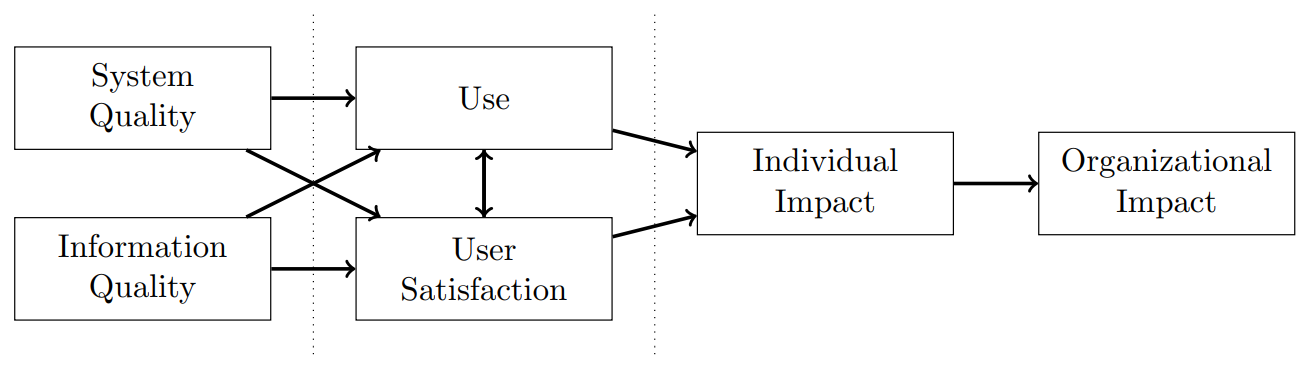
\includegraphics[width=\textwidth]{related_work/deloneMclean.png}
        \caption{Community Information Systems Success Model by DeLone and McLean \cite{DeMc92}}
        %13!!!!
      \end{figure}
    \end{column}
  \end{columns}
\end{frame}

\section{Concept}
\subsection{Use Case}
\begin{frame}{Mensa Communities}
  \begin{itemize}
    \item Community of people frequently visiting the mensa
    \item Community consists of students and university employees
    \item Similar to the concept of Community of Practice %share a concern: food at the canteen. And Interact regularly: Students argumenting on which mensa is the best?? Freqwuent visits to mensa
    \item Different community levels:
          \begin{itemize}
            \item Top level: all mensa frequenteers in Germany
            \item Intermediate level: all mensa frequenteers for a University
            \item Low level: individual circle of friends, which frequent the canteen together %Members can belong to different circles of friends->overlapping
          \end{itemize}
  \end{itemize}
\end{frame}



\section{Evaluation}

\begin{frame}{Overview}
  \begin{itemize}
    \item Research question: What is the impact of the chatbot on the community
          \begin{itemize}
            \item Collaboration
            \item Success awareness
            \item Mobility
          \end{itemize}
  \end{itemize}
\end{frame}

\begin{frame}{Main tasks}
  \begin{enumerate}
    \item Use the bot to get the menu and make a review
    \item Make visualizations of success factors
    \item Modify the success model of the commmunity
  \end{enumerate}
  
If you have the Slack app  installed (or want to install it) on your phone, you can use you phone to do the evaluation
    

\end{frame}


\begin{frame}{Joining the Slack workspace}
  \begin{columns}
    \begin{column}[]{0.7\textwidth}
      \begin{itemize}
        \item Use the following link \\
         \url{https://join.slack.com/t/mensacommunity/shared_invite/zt-nf09nfmb-EsChPf76BwKsUUlaRJqFqw} to join the Slack workspace if you are not a member yet
        \item Use your email adress to sign in, or use Google Sign-in
         \begin{itemize}
          \item You might need to confirm your email adress
          \item Open your email account
          \item You should have received an email from Slack (Also check your spam folder)
          \item  Click the link inside the email. 
        \end{itemize}
       \item If you have the Slack app you can click the popup \emph{Open in Slack}
        \item If you do not possess the Slack app you can also use it in the browser.
        \item  Locate the bot in the left taskbar near the bottom under Apps
      \end{itemize}

    \end{column}
    \begin{column}[]{0.3\textwidth}
      \begin{figure}
        \centering
        
\includegraphics[width=0.9\textwidth]{frame.png}
      \end{figure}
    \end{column}
  \end{columns}
  
\end{frame}


\begin{frame}{Task 1 part 1}
  \begin{itemize}
    \item Locate the bot in the left taskbar near the bottom under Apps
    \item Write a greeting message (e.g. Hello)
    \item You can type \emph{help} to see a list of the capabilities of the bot
    \item Ask the bot to get the menu for your local mensa
    \begin{itemize}
      \item Mensas might be closed
      \item Try using Aachen, Mensa Academica or Aachen, Mensa Vita
    \end{itemize}
    \item The bot might ask you, if you want to set a default city
  \end{itemize}
\end{frame}

\begin{frame}{Task 1 part 2}
  \begin{itemize}
    \item Ask the bot to make a review (e.g. I want to add a review)
    \item The review process should now be starting 
    \item The bot will ask you a series of questions
    \begin{itemize}
      \item Which mensa you went to and which meal you had (e.g. I went to Aachen, Mensa Academica and had the Klassiker) 
      \item Pay attention to write the category of the dish in the same manner that it is displayed on the menu
      \item How many stars out of 5 you would give your meal
      \item The bot will ask you to leave a comment
    \end{itemize}
  \end{itemize}
\end{frame}

\begin{frame}{Task 2}
  \begin{itemize}
    \item Ask the bot to make a review Visualization
    \item The bot will ask for a measure. Ask the bot to list all measures
    \item Choose one of the measures 
    \item The bot will respond with the appropriate visualization
  \end{itemize}
\end{frame}

\begin{frame}{Task 3}
  \begin{itemize}
    \item Use the bot to get the success model
    \item Aks the bot to update the success model
    \item The bot will ask you to choose which success dimension you want to edit
    \item Choose a dimension by providing a number
    \item The bot will now ask you which success factor you want to edit
    \item Choose one by providing a number or add one by choosing an name for the factor
    \item Select one of the measures to add it to your factor. 
    \item The bot will now add the factor to the model.
    \item You can verify that it was added by typing "get the success model" into the chat
    \item You can also visualize your new measure in the same way as described in Task 2 on the previous slide
  \end{itemize}
\end{frame}

\section{Feedback}
\begin{frame}
  \begin{itemize}
    \item Feedback?
    \item Please fill out the following survey: \url{https://docs.google.com/forms/d/e/1FAIpQLSfHn9kDKvCtccT3wqAOMIe-whJYlDP1l2pYTJinhNhZiNunTA/viewform?usp=sf_link}
    \end{itemize}
\end{frame}

%------------------------------------------------

\begin{frame}
\frametitle{References}
\footnotesize{
	\bibliographystyle{apalike}
	\bibliography{../../bibliography/bibliography}
}
\end{frame}

%------------------------------------------------

\begin{frame}
\Huge{\centerline{The End}}
\end{frame}

%----------------------------------------------------------------------------------------

\end{document} 
